\begin{tikzpicture}[
tectext/.style = {
    append after command={% <= for the border
        \pgfextra{%
            \begin{pgfinterruptpath}\begin{pgfonlayer}{foreground}
            \draw[-,line width=\pgflinewidth] let \p1=($(\tikzlastnode.south west)$),
                \p2=($(\tikzlastnode.south east)$) in
                (\p1) -- (\p2);
            \end{pgfonlayer}\end{pgfinterruptpath}
        }
    }
}]

\node[anchor=south west,inner sep=0] (image) at (0,0) {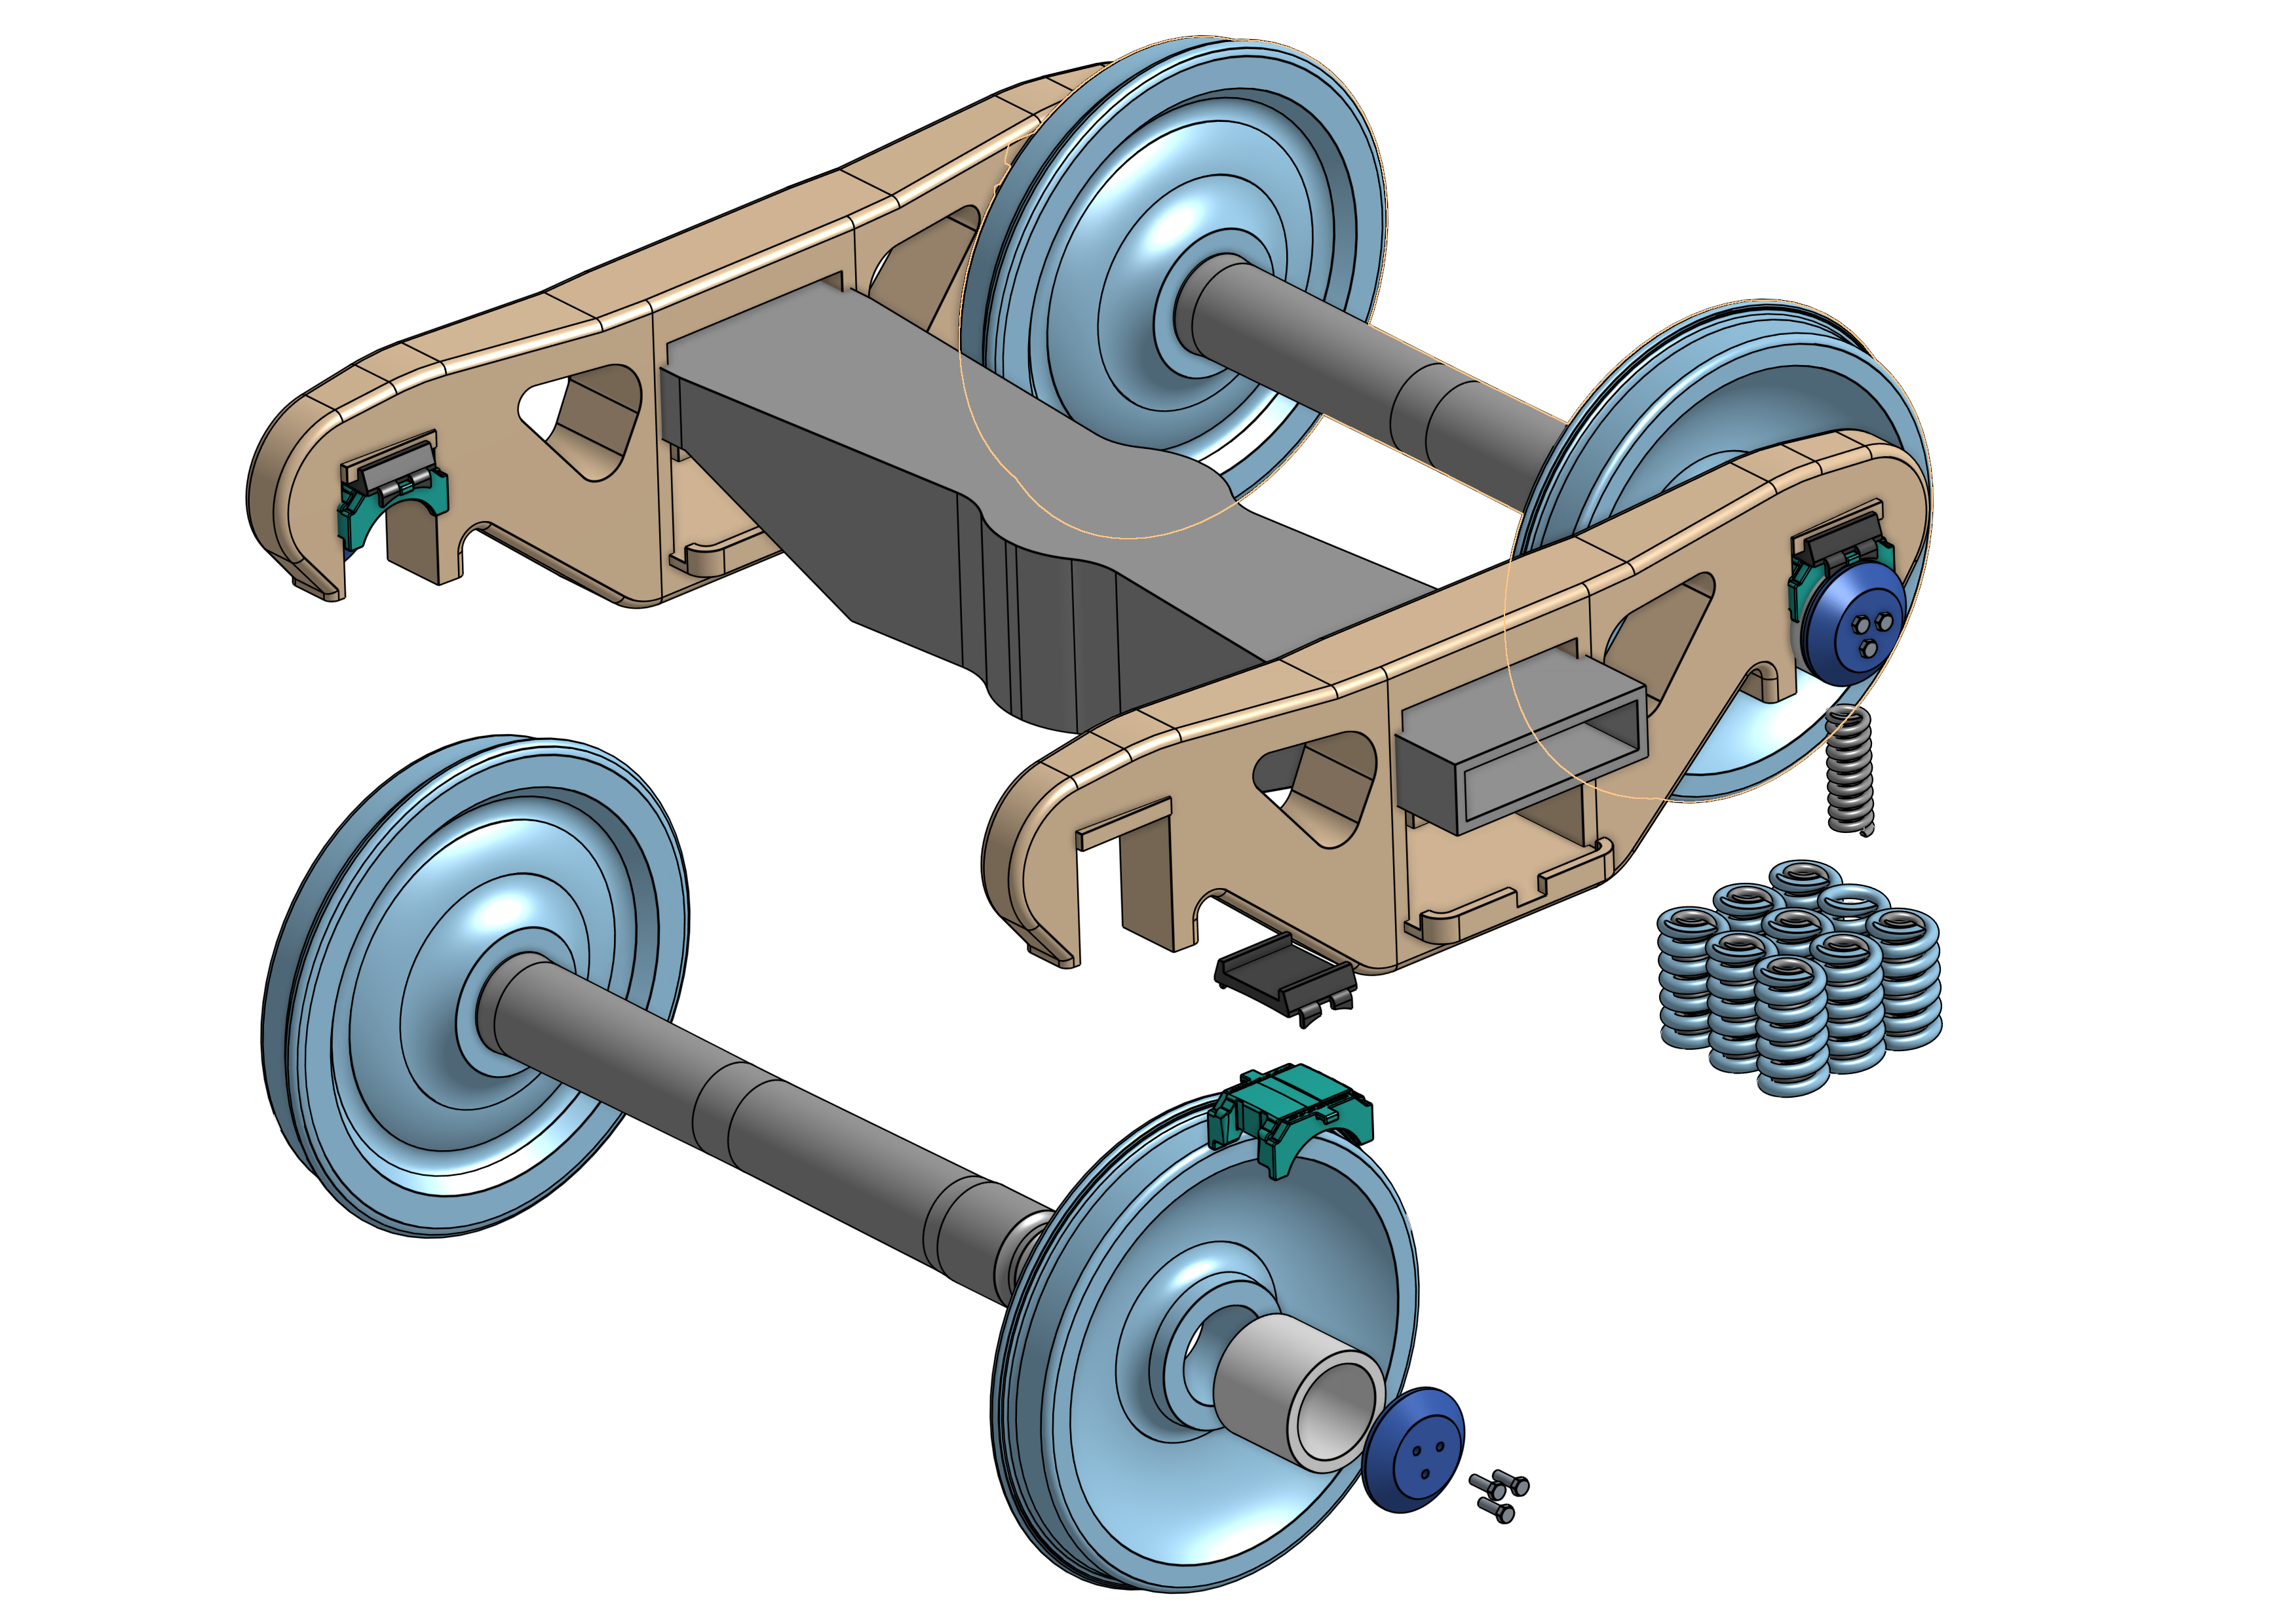
\includegraphics[width=0.6\columnwidth]{Cap_2/Figuras/truque_explodido_new.png}};
    \begin{scope}[x={(image.south east)},y={(image.north west)}]
        % \draw[help lines,step=.1] (0,0) grid (1,1);
        % \draw[help lines,step=.025,dashed] (0,0) grid (1,1);
        \draw[stealth-](0.53,0.15) -- (0.4,0.08) node[tectext,anchor=south east]{Caixa de mancal};
        \draw[stealth-](0.53,0.3) -- (0.4,0.18) node[tectext,anchor=south east,fill=white,fill opacity=0.6,text opacity=1]{Adaptador};
        \draw[stealth-](0.54,0.40) -- (0.4,0.38) node[tectext,anchor=south east,fill=white,fill opacity=0.6,text opacity=1]{Sapata};
        \draw[stealth-](0.44,0.94) -- (0.26,1.05) node[tectext,anchor=south east,]{Lateral};
        \draw[stealth-](0.49,0.49) -- (0.225,0.575) node[tectext,anchor=south east]{Pedestal}; 
        \draw[stealth-](0.48,0.70) -- (0.26,0.87) node[tectext,anchor=south east]{Travessa};
        \draw[stealth-](0.80,0.8) -- (0.95,0.87) node[tectext,anchor=south west]{Rodeiro};
        \draw[stealth-](0.81,0.38) -- (0.95,0.28) node[tectext,anchor=south west,text width=4cm]{{Molas da suspensão secundária}};
        \draw[ultra thick, rounded corners,dashed] (.50,.45) rectangle (.69,0.055) 
        node[anchor=north west,shift={(-0.08,0)},text width=1] {{Suspensão \\ {primária}}};
    \end{scope}
\end{tikzpicture}